\documentclass[UTF8,fontset=none,12pt]{ctexart}

\setCJKmainfont{Songti SC}
\setCJKsansfont{PingFang SC}
\setCJKmonofont{Songti SC}

\usepackage[a4paper,margin=2.35cm]{geometry}
\usepackage{amsmath,amssymb,amsthm,mathtools,bm}
\usepackage{graphicx}
\usepackage{float}
\usepackage{booktabs}
\usepackage{array}
\usepackage{enumitem}
\usepackage[hidelinks]{hyperref}

\newcommand{\epsmach}{\varepsilon_{\mathrm{machine}}}

\title{数值线性代数\quad 第 22 讲：高斯消去法的稳定性}
\author{Lloyd N. Trefethen、David Bau III\quad 中文阅读版}
\date{}

\begin{document}
\maketitle
\pagestyle{plain}

带部分选主元的高斯消去法对某些矩阵会表现出爆炸性的
不稳定性，但在实践中却通常十分稳定。这个看似矛盾的现象，
可以由统计观点得到解释。

\section*{$L$ 和 $U$ 的大小与稳定性}

数值线性代数中大多数算法的稳定性分析都相当直接，尤其是那些
建立在酉变换基础上的算法。可是，带部分选主元的高斯消去法的
稳定性分析要复杂得多；自 20 世纪 50 年代以来，它一直是数值分析
中的困难问题之一。这也是本书把高斯消去法放到后半部分讨论的原因之一。

第 20 讲的公式 (20.9) 给出了一个不带选主元的高斯消去法不稳定的
二阶矩阵例子。在那个例子中，因子 $L$ 含有一个大小为 $10^{20}$ 的
条目。若利用 $L$ 求解方程组，舍入误差的相对量级为
$\epsmach$，于是绝对误差的量级为 $\epsmach\times 10^{20}$；
结果的精度自然会被彻底破坏。

这个例子在某种意义上完全具有一般性。带选主元或不带选主元的
高斯消去法，只有在因子 $L$ 或 $U$ 相对于 $A$ 过大时才可能不稳定。
因此，从稳定性的角度看，选主元的目的就是确保 $L$ 和 $U$ 不会太大。
只要消去过程中出现的所有中间量都处于可控制的范围内，它们产生的
舍入误差就会很小，算法也就是向后稳定的。

下面的定理把这个想法精确化。定理针对不带选主元的高斯消去法表述，
但只要把 $A$ 理解为经过适当行置换和/或列置换的原始矩阵，
它同样适用于带选主元的情形。

\paragraph{定理 22.1.}
设非奇异矩阵 $A\in\mathbb{C}^{m\times m}$ 的分解
$A=LU$ 由算法 20.1 在满足公理 (13.5) 和 (13.7) 的计算机上、
使用不带选主元的高斯消去法计算得到。若 $A$ 存在 $LU$ 分解，
则当 $\epsmach$ 足够小时，浮点分解能够成功完成（不会遇到零主元），
并且计算得到的矩阵 $\widetilde L$ 和 $\widetilde U$ 满足
\begin{equation}
 \widetilde L\widetilde U=A+\delta A,\qquad
 \frac{\|\delta A\|}{\|L\|\,\|U\|}=O(\epsmach),
 \qquad \delta A\in\mathbb{C}^{m\times m}.
 \tag{22.1}
\end{equation}

和本书中的其他稳定性估计一样，这里不声称
$\widetilde L-L$ 或 $\widetilde U-U$ 很小；我们只关心
$\widetilde L\widetilde U-LU$ 的大小。乍看之下，(22.1) 似乎与
公式 (16.3)、(17.3) 等估计相同，但它的不同之处在于分母是
$\|L\|\,\|U\|$，而不是 $\|A\|$。如果
$\|L\|\,\|U\|=O(\|A\|)$，那么 (22.1) 说明高斯消去法向后稳定；
若不满足这个条件，则应当预期向后不稳定。

不带选主元的高斯消去法可能产生无界大的 $L$ 和 $U$。
这个算法按任何标准都不稳定，本讲不再讨论它；从现在起，
我们只讨论带部分选主元的高斯消去法。

\section*{增长因子}

在带部分选主元的高斯消去法中，每一次选主元都是在一列中取最大值，
因此所得矩阵 $L$ 在对角线下方的条目都满足
$|l_{ij}|\le 1$。这意味着在任意范数下都有 $\|L\|=O(1)$。
于是，对于带部分选主元的高斯消去法，(22.1) 化为
\begin{equation*}
 \frac{\|\delta A\|}{\|U\|}=O(\epsmach).
\end{equation*}
因此，只要 $\|U\|=O(\|A\|)$，算法就是向后稳定的。

这个结论有一种更形象的标准表述。高斯消去法把满矩阵 $A$
化为上三角矩阵 $U$；稳定性所关心的，就是在这个过程中矩阵条目
是否被放大。定义 $A$ 的增长因子为
\begin{equation}
 \rho=\frac{\displaystyle\max_{i,j}|u_{ij}|}
 {\displaystyle\max_{i,j}|a_{ij}|}.
 \tag{22.2}
\end{equation}
若 $\rho$ 为 $O(1)$，说明条目没有明显增长，消去过程是稳定的；
若 $\rho$ 很大，则应当预期不稳定。具体地，由 $\|L\|=O(1)$
以及 (22.2) 给出的 $\|U\|=O(\rho\|A\|)$，可得下述定理。

\paragraph{定理 22.2.}
设矩阵 $A\in\mathbb{C}^{m\times m}$ 的分解 $PA=LU$ 由算法 21.1
在满足公理 (13.5) 和 (13.7) 的计算机上、使用带部分选主元的
高斯消去法计算得到。则计算所得的矩阵 $\widetilde P$、
$\widetilde L$ 和 $\widetilde U$ 满足
\begin{equation}
 \widetilde L\widetilde U=\widetilde P A+\delta A,\qquad
 \frac{\|\delta A\|}{\|A\|}=O(\rho\epsmach),
 \qquad \delta A\in\mathbb{C}^{m\times m},
 \tag{22.3}
\end{equation}
其中 $\rho$ 是 $A$ 的增长因子。如果对每个 $i>j$ 都有
$|l_{ij}|<1$，也就是精确算术中选主元时不存在并列最大值，
那么当 $\epsmach$ 足够小时，$\widetilde P=P$。

高斯消去法向后稳定吗？根据定理 22.2 和第 14 讲的向后稳定性
定义，如果对给定维数 $m$ 的所有矩阵，$\rho=O(1)$ 且这个界
对矩阵是一致的，答案是肯定的；否则是否定的。

现在，复杂性开始出现。

\section*{最坏情形的不稳定性}

对于某些矩阵 $A$，即使选主元有益，增长因子 $\rho$ 仍然可能很大。
例如，考虑下列形式的矩阵（这里展示 $5\times5$ 情形）：
\begin{equation}
 A=
 \begin{bmatrix}
 1&0&0&0&1\\
 -1&1&0&0&1\\
 -1&-1&1&0&1\\
 -1&-1&-1&1&1\\
 -1&-1&-1&-1&1
 \end{bmatrix}.
 \tag{22.4}
\end{equation}
第一步不需要选主元，但最后一列中的第 2、3、$\ldots$、$m$ 个
条目会从 $1$ 加倍为 $2$。之后每一次消去都会再发生一次加倍。
最后得到
\begin{equation}
 U=
 \begin{bmatrix}
 1&0&0&0&1\\
 0&1&0&0&2\\
 0&0&1&0&4\\
 0&0&0&1&8\\
 0&0&0&0&16
 \end{bmatrix}.
 \tag{22.5}
\end{equation}

对应的 $PA=LU$ 分解在这个例子中为
\begin{equation*}
\begin{bmatrix}
 1&0&0&0&1\\
 -1&1&0&0&1\\
 -1&-1&1&0&1\\
 -1&-1&-1&1&1\\
 -1&-1&-1&-1&1
\end{bmatrix}
=
\begin{bmatrix}
 1&0&0&0&0\\
 -1&1&0&0&0\\
 -1&-1&1&0&0\\
 -1&-1&-1&1&0\\
 -1&-1&-1&-1&1
\end{bmatrix}
\begin{bmatrix}
 1&0&0&0&1\\
 0&1&0&0&2\\
 0&0&1&0&4\\
 0&0&0&1&8\\
 0&0&0&0&16
\end{bmatrix}.
\end{equation*}
对于这个 $5\times5$ 矩阵，增长因子是 $\rho=16$。
对于同样形式的 $m\times m$ 矩阵，
\[
 \rho=2^{m-1}.
\]
这是 $\rho$ 可能达到的最大值，见习题 22.1。

量级为 $2^m$ 的增长因子意味着大约损失 $m$ 个精度比特，
这对实际计算是灾难性的。典型计算机用 64 个比特表示浮点数，
但人们一直在求解几百乃至几千维的矩阵问题；损失 $m$ 个比特
显然是无法接受的。

这把我们带到了一个尴尬的地方。在讨论带选主元的高斯消去法时，
这是全书唯一一次：第 14 讲给出的稳定性定义失效了。根据那些定义，
决定稳定性或向后稳定性的唯一条件，是对每个固定维数 $m$ 的所有矩阵
都存在一个一致适用的界；并不要求这个界关于 $m$ 也一致。
在这里，对每个 $m$ 都有涉及常数 $2^{m-1}$ 的一致界。
所以，按照我们的形式定义，高斯消去法是向后稳定的。

\paragraph{定理 22.3.}
按照第 14 讲的定义，带部分选主元的高斯消去法是向后稳定的。

然而，鉴于 $2^{m-1}$ 对实际的 $m$ 来说极其巨大，
这个结论显然荒谬。

在本讲剩余部分，请读者暂时放下形式化的稳定性定义，
接受一种更非正式、也更通常的用词方式。对某些矩阵而言，
高斯消去法确实会爆炸性不稳定；使用 MATLAB、UNPACK、LAPACK
或其他可靠软件包进行数值实验即可确认这一点（习题 22.2）。

\section*{实践中的稳定性}

如果高斯消去法会不稳定，它为什么仍然如此著名、如此常用？
这里涉及的并不只是定义造成的假象，而是算法行为的一个基本事实：
尽管存在类似 (22.4) 的矩阵，带部分选主元的高斯消去法在实践中
却几乎总是稳定的。像 (22.5) 那样巨大的因子 $U$ 从未出现在
真实应用中。五十年的计算经验中，人们还没有发现自然环境下产生的
矩阵问题会激发这种爆炸性不稳定。

这确实很奇怪：一个对某些矩阵失效的算法，为什么在实践中能够
完全值得信赖？答案似乎是，虽然某些矩阵会导致不稳定，
但它们在所有矩阵中所占的比例极小；正是统计原因，使它们在实践中
几乎“从不”出现。

考察随机矩阵可以进一步了解这一现象。当然，应用中出现的矩阵
并非通常意义上的随机矩阵，它们具有各种特殊性质。若要把它们描述为
来自某个分布的随机样本，这个分布一定会非常奇特；期待某个特定的
随机矩阵分布在定量意义上准确匹配实际矩阵的行为，是不合理的。

不过，这里要解释的现象并不依赖精确的数值。应用中大增长因子的矩阵
极其罕见；如果能够证明，在某个定义明确的随机矩阵类中它们也极其罕见，
那么背后的机制必定是相同的。这个论证不要求两个“极其罕见”的度量
相差不超过某个固定因子，例如 2、10 或 100。

图 22.1 和图 22.2 展示了习题 12.3 中随机矩阵的实验：
每个条目都是均值为 0、标准差为 $m^{-1/2}$ 的实正态分布独立样本。
图 22.1 中，对不同维数的一组随机矩阵进行分解，并把增长因子画成
散点图；只有两个矩阵的增长因子达到 $m^{1/2}$ 那么大。
图 22.2 中，分别对 $m=8,16,32$ 的一百万个矩阵进行分解，
将增长因子按宽度为 0.2 的区间分箱，再画出概率密度。
增长因子的概率密度似乎随 $\rho$ 指数下降。在这三百万个矩阵中，
尽管理论上增长因子最大可以达到
$2{,}147{,}483{,}648$，实际遇到的最大值却只有 11.99。

采用其他概率分布也会得到类似结果，例如从 $[-1,1]$ 均匀分布中
抽取条目（习题 22.3）。如果随机抽取十亿个矩阵，几乎肯定也找不到
一个高斯消去法不稳定的矩阵。

\begin{figure}[H]
    \centering
    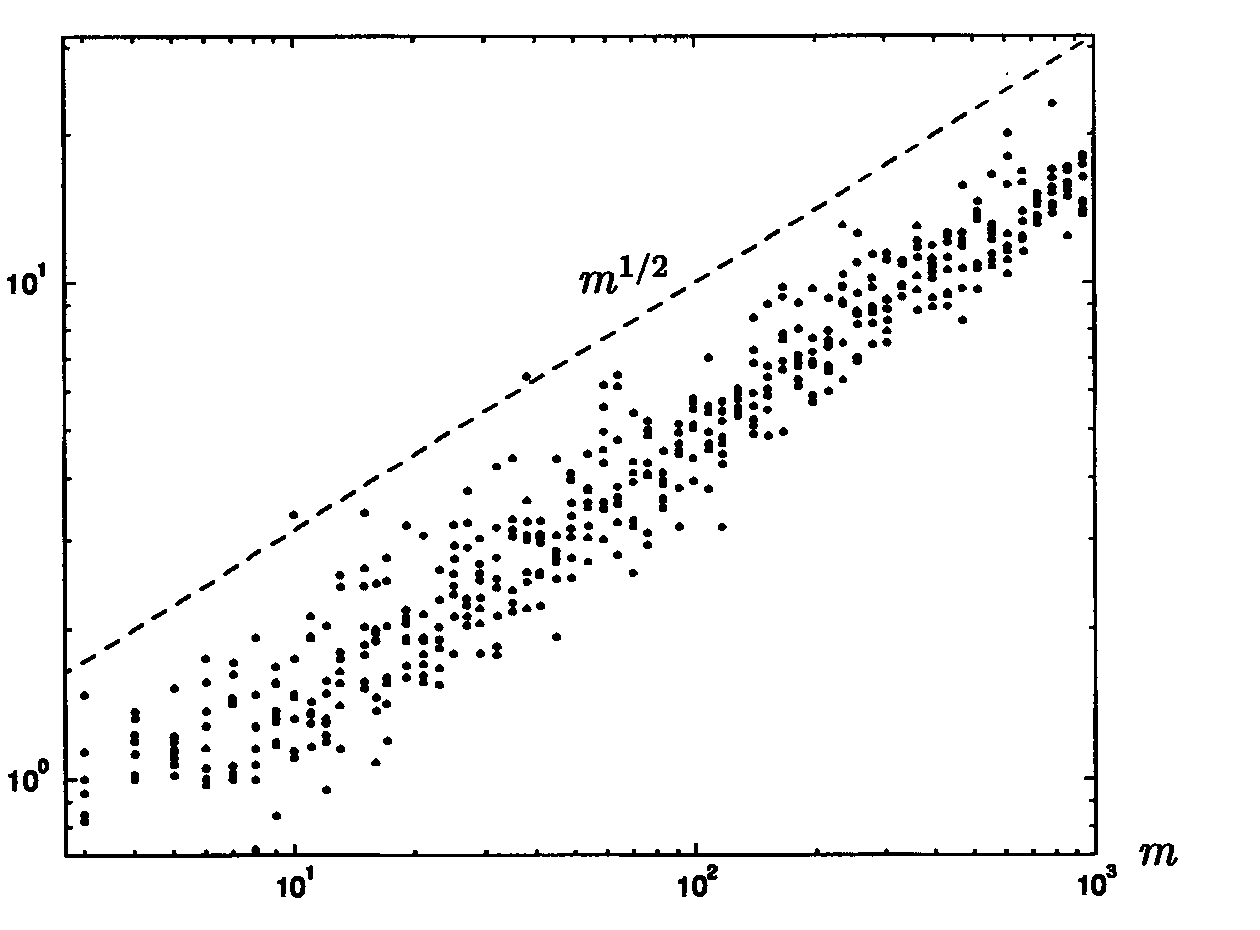
\includegraphics[width=0.88\linewidth]{../assets/figure-22-1.png}
    \caption{原书图 22.1：带部分选主元的高斯消去法作用于 496 个随机矩阵时的增长因子散点图。矩阵条目相互独立且服从正态分布。典型的 $\rho$ 量级为 $m^{1/2}$，远小于可能的最大值 $2^{m-1}$。}
\end{figure}

\begin{figure}[H]
    \centering
    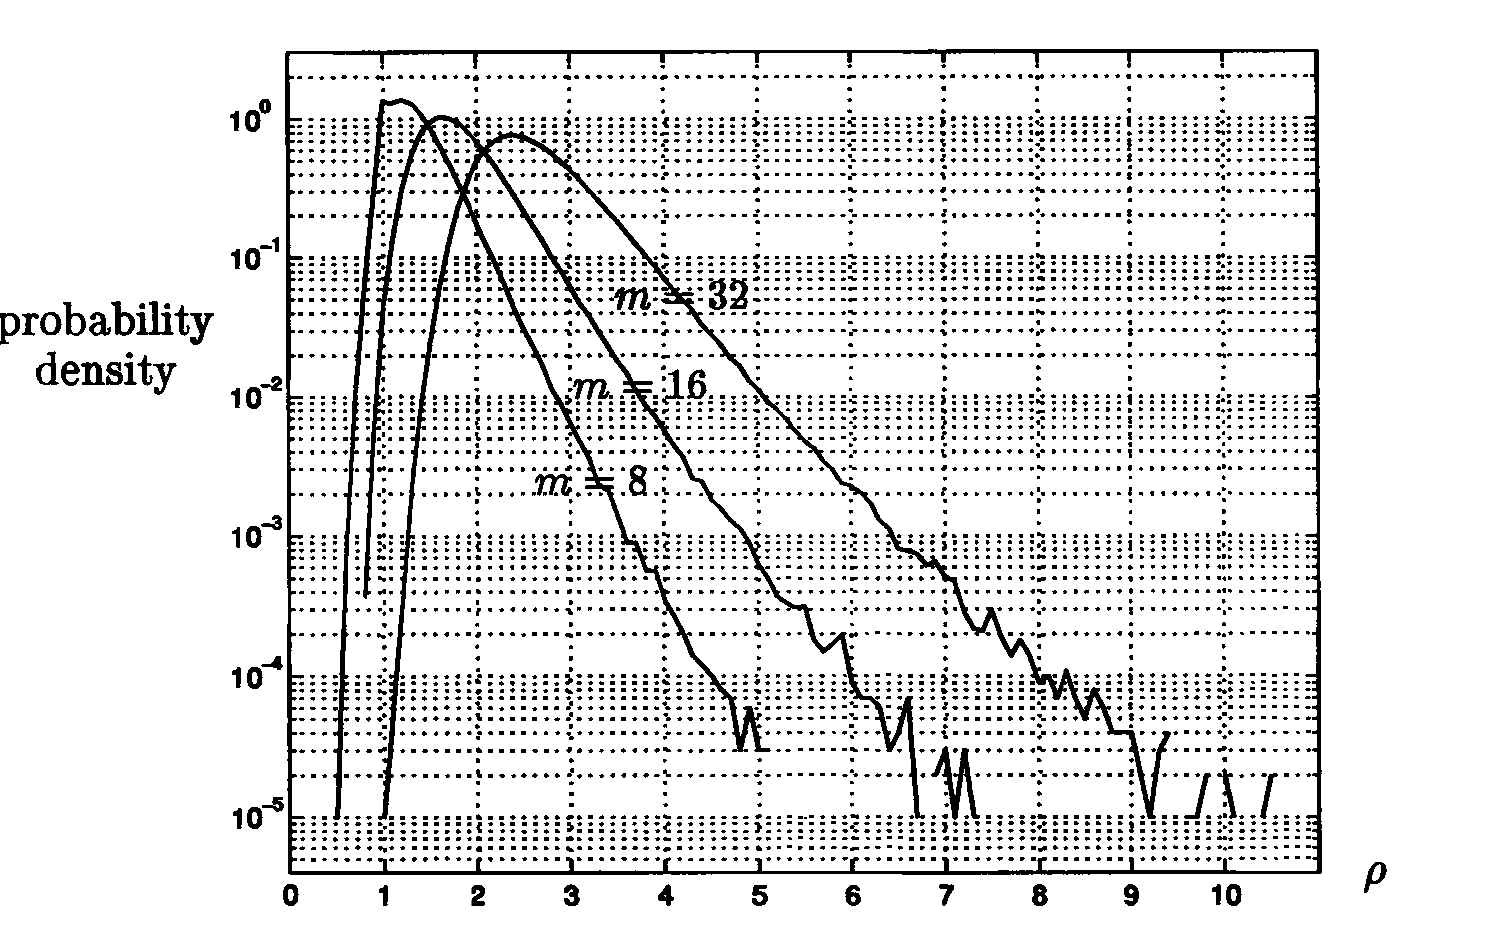
\includegraphics[width=0.88\linewidth]{../assets/figure-22-2.png}
    \caption{原书图 22.2：维数 $m=8,16,32$ 的随机矩阵增长因子概率密度。每种维数的样本量均为一百万。密度似乎随 $\rho$ 指数下降；曲线末端的抖动是有限样本量造成的。}
\end{figure}

\section*{解释}

若 $PA=LU$，则
\[
 U=L^{-1}PA.
\]
因此，如果把高斯消去法作用于矩阵 $A$ 时出现不稳定，即增长因子
$\rho$ 很大，那么 $L^{-1}$ 也必定很大。另一方面，随机三角矩阵
往往确实具有很大的逆；其大小随维数 $m$ 指数增长。对习题 12.3(d)
中的随机三角矩阵尤其如此；带部分选主元的高斯消去法产生的、对角线
为 1 且对角线下方条目绝对值不超过 1 的随机三角矩阵也具有这一性质。

然而，把高斯消去法应用于随机矩阵 $A$ 时，所得的因子 $L$ 一点也不像
随机三角矩阵。$L$ 的条目符号之间出现了相关性，使这些矩阵具有异常好的
条件性。$L^{-1}$ 的典型条目并没有指数增长，通常其绝对值还小于 1。
图 22.3 用一个维数 $m=128$ 的典型矩阵给出了这一现象的证据。

于是问题变成：为什么高斯消去法得到的 $L$ 几乎从不具有大的逆？

答案在于列空间。因为 $U$ 是上三角矩阵且 $PA=LU$，
$PA$ 与 $L$ 的列空间相同。这里的意思是：$PA$ 的第一列与 $L$ 的
第一列张成同一个空间，$PA$ 的前两列与 $L$ 的前两列张成同一个空间，
依此类推。如果 $A$ 是随机的，它的列空间具有随机方向；因此
$P^{-1}L$ 的列空间也应当具有随机方向。然而，这个条件与
$L^{-1}$ 很大是不相容的。可以证明，如果 $L^{-1}$ 很大，
那么 $L$ 的列空间，或任意置换矩阵 $P^{-1}L$ 的列空间，
必定以一种远离随机的特殊方式倾斜。

图 22.4 给出了证据。它显示了图 22.3 中同两个矩阵的连续列空间
“能量分布”在哪里。用来显示这一点的工具是 $Q$ 画像，其 MATLAB
命令为
\begin{equation}
 [Q,R]=\operatorname{qr}(A),\qquad
 \operatorname{spy}\bigl(\lvert Q\rvert>1/\sqrt{m}\bigr).
 \tag{22.6}
\end{equation}
这些命令先计算矩阵 $A$ 的 QR 分解，然后在 $Q$ 中每个满足
条目大于标准差 $m^{-1/2}$ 的位置画一个点。图中可以看出：
对于随机矩阵 $A$，即使经过行交换变成 $PA$，列空间仍然近似随机取向；
而对于产生大增长因子的矩阵 $A$，列空间的取向则远离随机。

很可能可以把这个论证定量化，从而证明：在随机矩阵中，
增长因子大于 $m^{1/2}$ 量级的事件是指数罕见的。更具体地，
对任意 $\alpha>1/2$ 和 $M>0$，当 $m$ 足够大时，
\[
 \Pr\{\rho>m^\alpha\}<m^{-M}.
\]
不过截至本书写作时，这样的定理还没有被证明。

我们总结带部分选主元的高斯消去法的稳定性。对于某些矩阵 $A$，
这个算法高度不稳定；但要发生不稳定，$A$ 的列空间必须以一种
非常特殊的方式倾斜，而这种方式在至少一类随机矩阵中是指数罕见的。
数十年的计算经验表明，具有这种倾斜列空间的矩阵在实际应用中极少出现。

\begin{figure}[H]
    \centering
    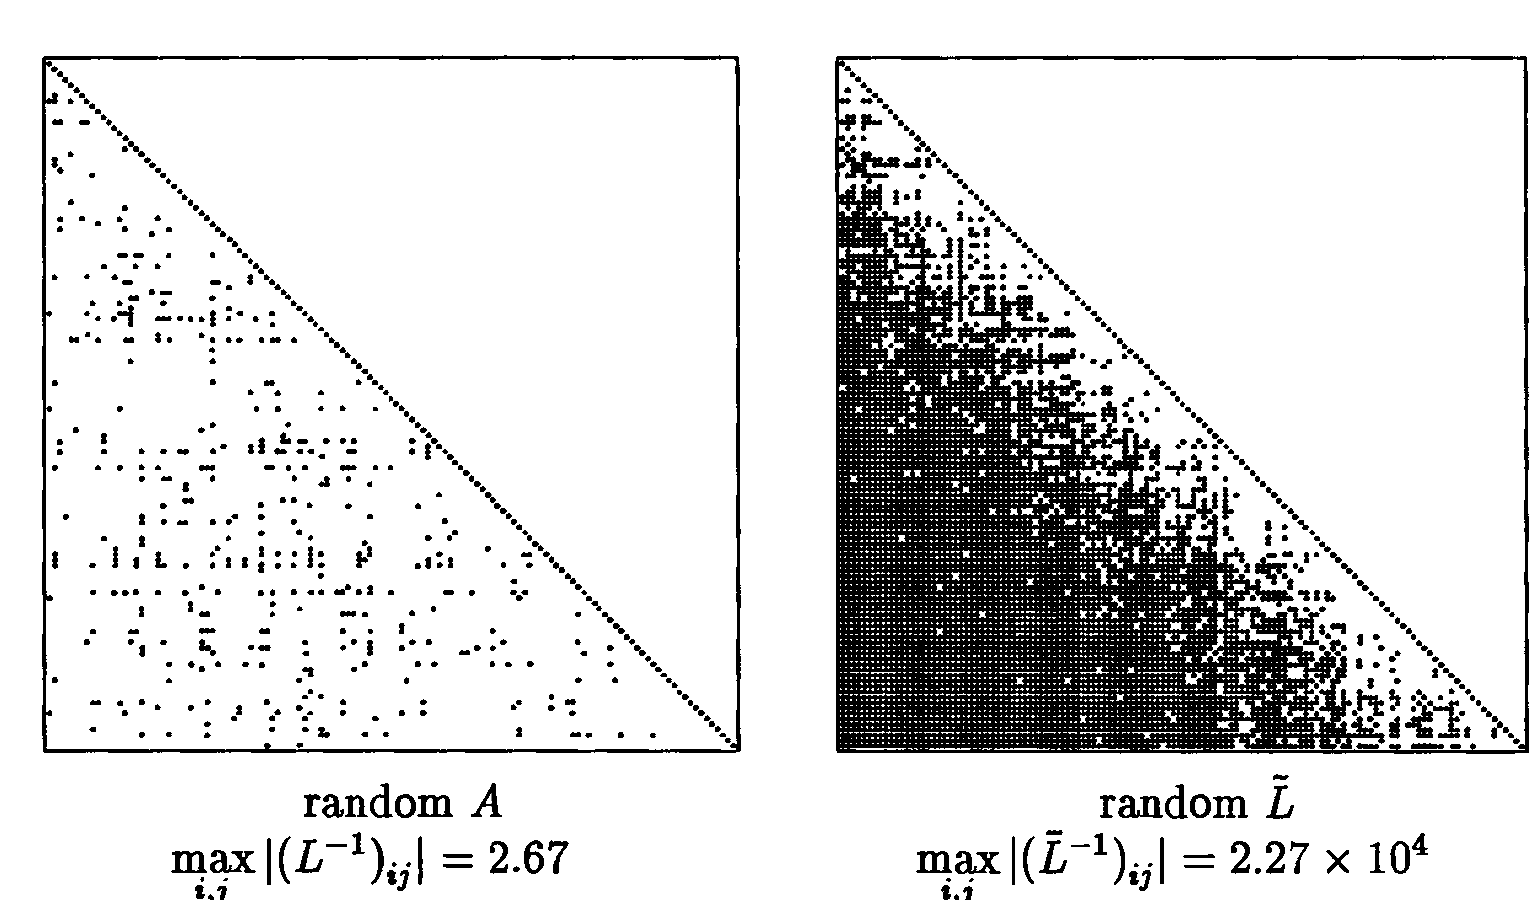
\includegraphics[width=0.90\linewidth]{../assets/figure-22-3.png}
    \caption{原书图 22.3：设随机的 $128\times128$ 矩阵 $A$ 满足 $PA=LU$。左图显示 $L^{-1}$，点表示绝对值大于等于 1 的条目；右图显示类似的 $\widetilde L^{-1}$，其中 $\widetilde L$ 与 $L$ 相同，只是其次对角线条目的符号被随机化。高斯消去法倾向于产生条件性异常良好的矩阵 $L$。}
\end{figure}

\begin{figure}[H]
    \centering
    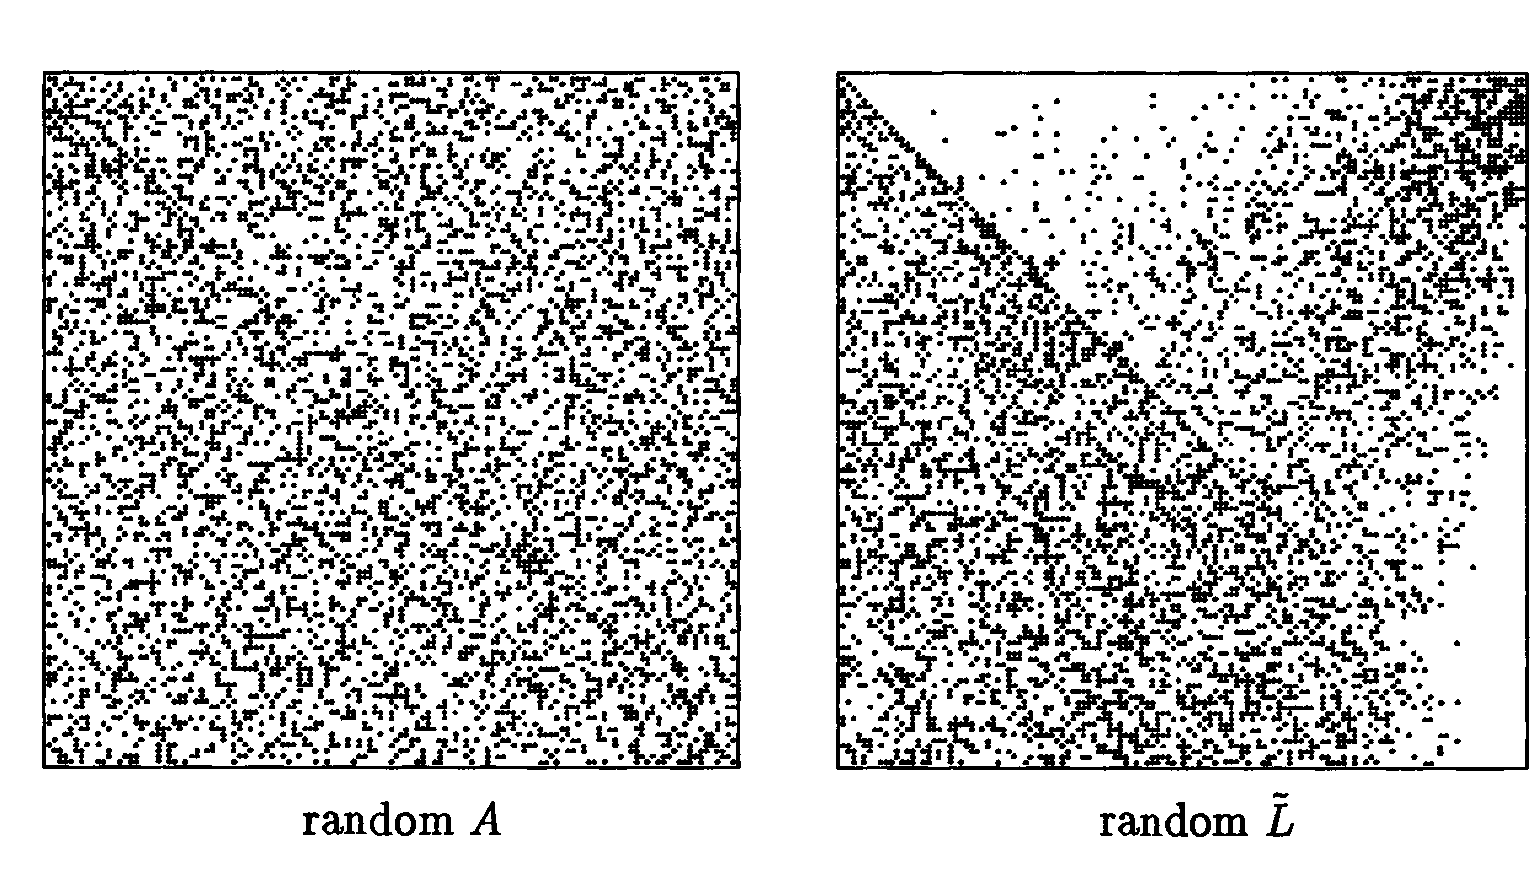
\includegraphics[width=0.90\linewidth]{../assets/figure-22-4.png}
    \caption{原书图 22.4：同两个矩阵的 $Q$ 画像 (22.6)。左图是置换为 $PA$ 后的随机矩阵 $A$，或等价地说是因子 $L$；右图是符号被随机化的矩阵 $\widetilde L$。在典型随机矩阵中，$\widetilde L$ 的列空间以图示方式倾斜是指数罕见的。}
\end{figure}

\section*{习题}

\begin{enumerate}[label=\textbf{22.\arabic*.},leftmargin=*]
    \item 证明：对任意矩阵 $A\in\mathbb{C}^{m\times m}$ 使用带部分选主元的高斯消去法时，增长因子 (22.2) 满足
    \[
    \rho\le 2^{m-1}.
    \]

    \item 对形如 (22.4) 的 $A$，使用带部分选主元的高斯消去法求解
    $60\times60$ 方程组 $Ax=b$。由于增长因子量级为 $2^{60}$，
    你是否观察到结果毫无用处？第一次尝试时可能观察不到这一点，
    因为 $A$ 的整数条目会阻止舍入误差出现。如果确实如此，
    请设法对问题作轻微修改，使增长因子保持相同或近似相同，
    并真正产生灾难性的舍入误差。

    \item 近似地（不必完全复现细节）重现本讲中的图，但使用
    $[-1,1]$ 均匀分布的随机矩阵条目，而不是正态分布条目。
    你是否看到显著差异？

    \item
    \begin{enumerate}[label=(\alph*),leftmargin=2em]
        \item 设 $PA=LU$（带部分选主元的 $LU$ 分解），且 $A=QR$
        （QR 分解）。描述 $L^{-1}$ 的最后一行与 $Q$ 的最后一列之间的关系。
        \item 证明：如果 $A$ 是条目相互独立且服从正态分布意义下的随机矩阵，
        那么它的列空间具有随机方向；特别地，$Q$ 的最后一列是随机单位向量。
        \item 综合 (a)、(b) 的结果，说明对随机矩阵 $A$ 进行高斯消去时，
        $L^{-1}$ 的最后一行具有什么性质。
    \end{enumerate}
\end{enumerate}

\end{document}
